The Decomposable-Informed Prior of Section~\ref{sec:misspec} carries one free parameter, the mixing weight $\lambda \in [0, 1]$ that interpolates between the BDMCMC default at $\lambda = 0$ and the Stage-1 PIP matrix at $\lambda = 1$. We report a sensitivity sweep over $\lambda$ on a representative set of topologies, with the reference probability fixed at $r_0 = 0.2$ to nest the BDMCMC default at the lower endpoint of the sweep, as motivated in Section~\ref{sec:sim}.

For each topology in $\{\text{chain}, \text{cycle}, \text{Erd\H{o}s--R\'enyi}\}$ and each Monte Carlo replicate $r \in \{1, \dots, 5\}$, we generate one dataset of $n = 500$ observations on $p = 10$ variables, run Stage-1 SAEM-MCMC once, and then sweep $\lambda$ over the eleven values $\{0.0, 0.1, \dots, 1.0\}$. Stage-2 BDMCMC reruns at every $\lambda$ with the DIP $p_{ij} = \lambda \, \text{PIP}_{ij} + (1 - \lambda)\,(0.2)$. Reusing the Stage-1 PIPs across the $\lambda$ grid within each unit isolates the effect of the mixing weight from sampling variability in Stage 1 and reduces wall-clock time by an order of magnitude. The three topologies cover the regime of interest: the chain is the canonical decomposable example; the cycle is the canonical non-decomposable example, generalizing the four-cycle of Figure~\ref{fig:decomposability_cliques} in Section~\ref{sec:theory}, with multiple minimal triangulations that make it the cleanest test of the DIP; and the Erd\H{o}s--R\'enyi graph adds variation in graph density across replicates and is non-decomposable in general.

\begin{figure}[H]
    \centering
    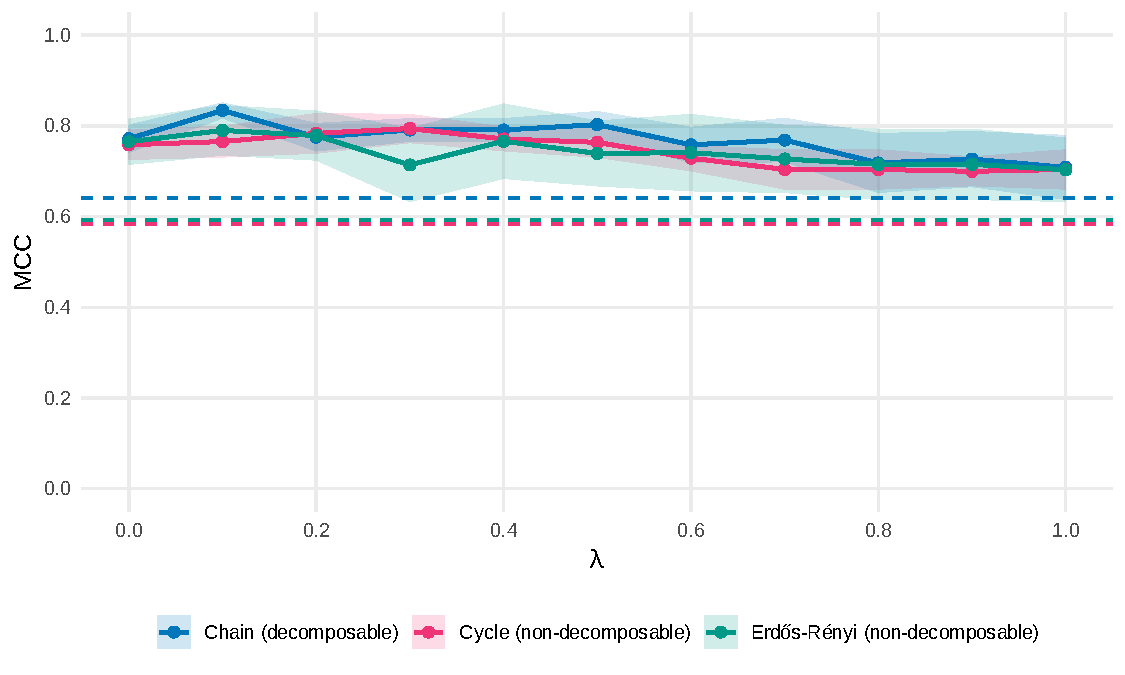
\includegraphics[width=0.85\linewidth]{../../2_analysis/output/figures/lambda_sensitivity.pdf}
    \caption{Stage-2 Matthews correlation coefficient (MCC) as a function of the DIP mixing weight $\lambda$, by topology, at $p = 10$, $n = 500$. Solid lines are means over five Monte Carlo replicates; ribbons mark $\pm 1$ standard error. Dashed lines are the Stage-1 estimator alone, which does not depend on $\lambda$ and is shown for reference.}
    \label{fig:lambda-sensitivity}
\end{figure}

All three Stage-2 curves substantially dominate the dashed Stage-1 reference lines throughout the sweep, by margins consistent with Section~\ref{sec:sim}: lifting the decomposability restriction is the binding contribution. The Stage-1 baselines in the figure are $0.53$ for chain, $0.55$ for cycle, and $0.37$ for Erd\H{o}s--R\'enyi at $p = 10$. Every Stage-2 curve sits well above its corresponding dashed line.

Within the Stage-2 family, the Stage-2 curves are jointly maximized at or near $\lambda = 0$. The chain peaks at $\lambda = 0$ with mean MCC $0.77$ and declines monotonically to $0.70$ at $\lambda = 1$. The cycle holds approximately flat at $0.76$--$0.75$ from $\lambda = 0$ to $\lambda = 0.4$, then declines to $0.70$ at $\lambda = 1$, with the largest drop concentrated in the upper half of the interval. The Erd\H{o}s--R\'enyi curve declines monotonically from $0.76$ at $\lambda = 0$ to $0.68$ at $\lambda = 1$. Standard-error ribbons remain narrow throughout; the ordering is robust to Monte Carlo variation.

The interpretation is the one Theorem~\ref{thm:concentration} predicts conditional on Stage-1's finite-sample convergence. With proper calibration $r_0 = 0.2$, the only mechanism by which $\lambda > 0$ can improve over the BDMCMC default is by transferring information about $E^*$ that Stage-1 has and the Stage-2 likelihood does not. At $n = 500$ with maximum partial correlation $\approx 0.13$, Stage-1's finite-sample PIPs on chain at $p = 10$ are accurate enough that a moderate $\lambda$ does not break the procedure, but they are not so accurate that mixing them in adds anything; on the cycle they carry the chord-edge inflation that \textcite{niu2020bayesian} characterize and that the DIP transfers to Stage 2 as a structural bias. The net effect across topologies is monotone degradation in $\lambda$ from a peak at $\lambda = 0$.

Two caveats apply to this empirical pattern. The boundary $\lambda = 0$ is at or near the recovery optimum on every topology in the sweep, but the gap to higher $\lambda$ is small ($0.06$--$0.08$ MCC at $\lambda = 1$ vs $\lambda = 0$, depending on topology) and reflects finite-sample noise in Stage-1's PIPs at our calibration ($n = 500$, $p = 10$, $\rho_{\max} \approx 0.13$) rather than asymptotic bias. A researcher with larger $n$ or a sparser $G^*$ should expect the curves to flatten further, and the within-Bayesian recovery cost of $\lambda > 0$ to shrink toward zero on truly decomposable truths.

The natural interpretation of $\lambda$ is therefore \textit{ex ante}, not \textit{ex post}. A researcher who has reason to believe that the underlying conditional-independence structure is approximately decomposable has principled reasons to set $\lambda > 0$. Decomposable graphs are more tractable than general ones, they admit closed-form normalizing constants and faster posterior sampling, and they inherit the asymptotic guarantees of Theorem~\ref{thm:concentration}. The empirical message of this appendix is that $\lambda = 0$ is the safe default for a practitioner with no such prior, not that $\lambda > 0$ is wrong for one who does. Used \textit{ex post}, the sweep cannot read off ``which edges depend on the decomposable approximation'' from the path of recovered structure as $\lambda$ rises: with enough data the Stage-2 likelihood washes out any reasonable prior, and the path collapses to a common posterior.

